\chapter{Additional Techniques for Solving ODEs}

\subsection*{Section~\protect{\ref{sec:VarConstS}} Nonconstant Coefficient
Linear Equations}
\rhead{sec:VarConstS}{NONCONSTANT COEFFICIENT LINEAR EQUATIONS}

\exer{c14.2.1a} The differential equation is linear and homogeneous.

\exer{c14.2.1c} The differential equation is linear and inhomogeneous.

\exer{c14.2.1e} The differential equation is linear and inhomogeneous.

\exer{c14.2.6a} \ans The solution to the initial value problem is
$x(t) = 2e^{\frac{1}{3}(t^3 - 1)} - 1$.

\soln By inspection $x(t) = -1$ is a solution to the inhomogeneous
equation.  The solution to the homogeneous equation $\dot{x}(t) = t^2x$ is
$x(t) = Ke^{H(t)}$, where
\[
H(t) = \int t^2dt = \frac{1}{3}t^3.
\]
So the general solution to the inhomogeneous equation is
\[
x(t) = Ke^{\frac{1}{3}t^3} - 1.
\]
Substitute the initial condition $x(1) = 1$ into this equation and
solve for $K = 2e^{-\frac{1}{3}}$.

\exer{c14.2.6c} \ans The solution to the initial value problem is
$x(t) = (3 - \cos t)\sqrt{t^2 + 1}$.

\soln By Theorem~\ref{thm:varpar}, the
solution to the initial value problem is $x(t) = c(t)e^{H(t)}$, where
$\frac{dx}{dt} = a(t)x + g(t)$.  So
\[
H(t) = \int_{t_0}^t a(\tau)d\tau = \int_0^t\frac{\tau}{\tau^2 + 1}d\tau
= \ln\sqrt{t^2 + 1}.
\]
\[
c(t) = \int_{t_0}^t g(\tau)e^{-H(\tau)}d\tau + x_0
= \int_0^t \sin(\tau)d\tau + 2
= 3 - \cos t.
\]

\exer{c14.2.11a} Using {\sf dfield5} we see in Figure~\ref{c14.2.11a} that
solutions are asymptotic to a line parallel to $x=\frac{1}{2}t$.

\begin{figure}[htb]
     \centerline{%
     \psfig{file=exfigure/fig17-1-11.eps,width=3.0in}}
        \exercap{c14.2.11a}
\end{figure} 
Using variation of parameters we find that the general solution to the
differential equation $\dot{x}=-2x+t$ is 
\[
x(t) = \frac{1}{2}\left(t-\frac{1}{2}\right) +Ke^{-2t}.
\]
As $t\to\infty$, the solution $x(t)$ approaches the straight line 
$x= \frac{1}{2}t-\frac{1}{4}$.

\exer{c14.2.11c}
Using {\sf dfield5} and variation of parameters we see in 
Figure~\ref{c14.2.11c} that solutions are asymptotic to the
periodic function $x=\frac{1}{5}(\cos t-2\sin t)$.
Using variation of parameters we find that the general solution to the
differential equation $\dot{x}=-2x+\sin t$ is 
\[
x(t) = \frac{1}{5}(\cos t-2\sin t) + Ke^{-2t}.
\]
As $t\to\infty$, the solution $x(t)$ approaches the function  
$x= \frac{1}{5}(\cos t-2\sin t)$ --- which is verified by the 
{\sf dfield5} calculations shown in Figure~\ref{c14.2.11c}.

\begin{figure}[htb]
     \centerline{%
     \psfig{file=exfigure/fig17-1-13.eps,width=3.0in}}
        \exercap{c14.2.11c}
\end{figure} 



\subsection*{Section~\protect{\ref{sec:LinInhomSys}} Variation of Parameters
for Systems}
\rhead{sec:LinInhomSys}{VARIATION OF PARAMETERS FOR SYSTEMS}

\exer{c14.3.1a} \ans The solution to the initial value problem is
\[
X(t) = \frac{1}{2}\cvectwo{te^t + e^t + 1}{te^t - e^t - 1}.
\]

\soln This system can be written as $\dot{X} = AX + G(t)$, where
\[
A = \frac{1}{2}\mattwo{1}{1}{1}{1} \AND G(t) = \vectwo{e^t}{0}.
\]
We can then solve the system by variation of parameters, as described in
Theorem~\ref{thm:varparsys}:

\paragraph{Step 1.} The eigenvalues of $A$ are $\lambda_1 = 0$ and
$\lambda_2 = 1$, with associated eigenvectors $v_1 = (1,-1)^t$ and
$v_2 = (1,1)^t$.  Thus, a basis of solutions to the homogeneous system
$\dot{X} = AX$ is
\[
X_1(t) = \vectwo{1}{-1} \AND X_2(t) = e^t\vectwo{1}{1}.
\]
\paragraph{Step 2.} To compute the vector $D(t)$, first compute
\[
Y(t)^{-1} = (X_1(t)|X_2(t))^{-1} = \cmattwo{1}{e^t}{-1}{e^t}^{-1} =
\frac{1}{2e^t}\cmattwo{e^t}{-e^t}{1}{1} =
\frac{1}{2}\cmattwo{1}{-1}{e^{-t}}{e^{-t}}.
\]
Then,
\[
D(t) = Y(t)^{-1}G(t) =
\frac{1}{2}\cmattwo{1}{-1}{e^{-t}}{e^{-t}}\vectwo{e^t}{0} =
\frac{1}{2}\vectwo{e^{t}}{1}.
\]
\paragraph{Step 3.} We find $c_1(0)$ and $c_2(0)$ using the initial
condition
\[
X_0 = c_1(0)X_1(0) + c_2(0)X_2(0).
\]
Therefore,
\[
\vectwo{1}{-1} = c_1(0)\vectwo{1}{-1} + c_2(0)\vectwo{1}{1}.
\]
Solve this system to obtain $c_1(0) = 1$ and $c_2(0) = 0$.  By definition,
$\dot{c_j} = d_j$.  Thus,
\[
c_1(t) = \int_{t_0}^td_1(\tau)d\tau + c_1(0)
= \frac{1}{2}\int_0^te^\tau d\tau + 1 = \frac{1}{2}(e^t + 1).
\]
\[
c_2(t) = \int_{t_0}^td_2(\tau)d\tau + c_2(0)
= \frac{1}{2}\int_0^td\tau = \frac{t}{2}.
\]
\paragraph{Step 4.} So, the solution to the initial value problem is
\[
X(t) = c_1(t)X_1(t) + c_2(t)X_2(t)
= \frac{1}{2}\left((e^t + 1)\vectwo{1}{-1} + \frac{t}{2}e^t\vectwo{1}{1}
\right).
\]

\exer{c17.3.3} \ans $X(t) = (\alpha_1+2t)X_1(t) + 
\left(\alpha_2-\frac{1}{3}t^3 \right)X_2(t)$.

\soln  Begin by verifying that $X_1=(1,t)^t$ and 
$X_2=(\frac{1}{t^2},-\frac{1}{t})^t$ solve the homogeneous
equation
\[
\frac{dX}{dt}= \mattwo{-\frac{1}{t}}{\frac{1}{t^2}}{1}{0}X.
\]
That is,
\[
\dot{X}_1 = \cvectwo{0}{1} \AND 
\mattwo{-\frac{1}{t}}{\frac{1}{t^2}}{1}{0}\cvectwo{1}{t} = 
\cvectwo{-\frac{1}{t}+\frac{1}{t}}{1} = \cvectwo{0}{1}
\]
and 
\[
\dot{X}_2 = \vectwo{-\frac{2}{t^3}}{\frac{1}{t^2}} \AND 
\mattwo{-\frac{1}{t}}{\frac{1}{t^2}}{1}{0}
\vectwo{\frac{1}{t^2}}{-\frac{1}{t}} = 
\cvectwo{-\frac{1}{t^3}-\frac{1}{t^3}}{\frac{1}{t^2}} 
= \vectwo{-\frac{2}{t^3}}{\frac{1}{t^2}}
\]

Next we look for a particular solution to the inhomogeneous equation of 
the form $X(t)=c_1(t)X_1(t)+c_2(t)X_2(t)$.  Equation~\Ref{e:D(t)} in
Theorem~\ref{thm:varparsys} states that $c_j$ satisfies
\[
\vectwo{\dot{c}_1}{\dot{c}_2} = (X_1|X_2)\inv \vectwo{1}{3t}.
\]
Now 
\[
(X_1|X_2)\inv = \mattwo{1}{\frac{1}{t^2}}{t}{-\frac{1}{t}}\inv = 
\frac{1}{2}\mattwo{1}{\frac{1}{t}}{t^2}{-t}
\]
It follows that 
\begin{eqnarray*}
\dot{c}_1 & = & 2 \\
\dot{c}_2 & = & -t^2.
\end{eqnarray*}
Integration yields
\begin{eqnarray*} 
c_1 & = & 2t\\
c_2 & = & -\frac{1}{3}t^3.
\end{eqnarray*}
Adding the general solution to the homogeneous equation to the specific
solution to the inhomogeneous equation yields the general solution to the
inhomogeneous equation.



\subsection*{Section~\protect{\ref{S:wronskian}} The Wronskian}
\rhead{S:wronskian}{THE WRONSKIAN}

\exer{c14.4.1a} \ans The Wronskian is $W(t) = t^2 + 1$.

\soln $W(t) = \det(Y(t)) = \det\mattwo{t}{1}{-1}{t} = t^2 + 1$.

\exer{c14.4.1c} \ans The Wronskian is $W(t) = te^t(1 - t)$.

\soln
\[
W(t) = \det(Y(t)) = \det\cmatthree{0}{t}{e^t}{1}{t}{te^t}{t}{t}{t^2e^t}
= te^t - t^2e^t.
\]

\exer{c14.w.2} Equation \Ref{L:Wronskian}
states that the Wronskian for solutions to $\dot{X} = AX$ is
\[
W(t) = e^{\int_0^t\trace(A(\tau))d\tau}W(0).
\]
If $\dot{X} = AX$ is a linear constant coefficient system, then $A$ is not
time-dependent, so $\trace(A(t)) = \trace(A)$ for all $t$.  Thus,
\[
\int_0^t\trace(A(\tau))d\tau = \int_0^t\trace(A)d\tau = \trace(A)t,
\]
and $W(t) = e^{\trace(A)t}W(0)$, as desired.

\exer{c14.w.3b} \ans The Wronskian is $W(t) = -2e^{4t}$.

\soln First, find that $A$ has eigenvalues $\lambda_1 = 5$ and
$\lambda_2 = -1$ with corresponding eigenvectors $v_1 = (1,1)^t$ and
$v_2 = (1,-1)^t$.  Thus, the vectors $X_1(t) = e^{5t}(1,1)^t$ and
$X_2(t) = e^{-t}(1,-1)^t$ are linearly independent solutions to
$\dot{X} = AX$.  So the matrix whose columns are solutions to this
system is
\[
Y(t) = \mattwo{e^{5t}}{e^{-t}}{e^{5t}}{-e^{-t}}.
\]
Compute the right hand side of \Ref{E:ccw}:
\[
W(t) = e^{\trace(A)t}W(0) = e^{4t}\det(Y(0)) = -2e^{4t}.
\]
To verify that this result is correct, compute the left hand side of
\Ref{E:ccw} by definition of the Wronskian:
\[
W(t) = \det(Y(t)) = -2e^{4t}.
\]



\subsection*{Section~\protect{\ref{S:RO}} Higher Order Equations}
\rhead{S:RO}{HIGHER ORDER EQUATIONS}

\exer{c14.3.2a} \ans The solution to the initial value problem is 
$x(t) = t^5$.

\soln The second order equation can be written as a system
$\dot{X} = A(t)X + G(t)$, where
\[
A(t) = \mattwo{0}{1}{\frac{6}{t^2}}{0} \AND G(t) = \cvectwo{0}{14t^3}.
\]
We can then solve the system by variation of parameters, as described in
Theorem~\ref{thm:varparsys}:

\paragraph{Step 1.} The hint states that
a basis of solutions to the homogeneous system
$\dot{X} = A(t)X$ is
\[
X_1(t) = \vectwo{t^3}{3t^2} \AND X_2(t) =
\vectwo{\frac{1}{t^2}}{-\frac{2}{t^3}}.
\]
\paragraph{Step 2.} To compute the vector $D(t)$, first compute
\[
Y(t)^{-1} = (X_1(t)|X_2(t))^{-1} =
\cmattwo{t^3}{\frac{1}{t^2}}{3t^2}{-\frac{2}{t^3}}^{-1} =
\frac{1}{5}\cmattwo{\frac{2}{t^3}}{\frac{1}{t^2}}{3t^2}{-t^3}.
\]
Then,
\[
D(t) = Y(t)^{-1}G(t) =
\frac{14}{5}\cvectwo{t}{-t^6}.
\]
\paragraph{Step 3.} We find $c_1(-1)$ and $c_2(-1)$ using the initial
condition
\[
X_0 = c_1(-1)X_1(-1) + c_2(-1)X_2(-1).
\]
Therefore,
\[
\vectwo{-1}{5} = c_1(-1)\vectwo{-1}{3} + c_2(-1)\vectwo{1}{2}.
\]
Solve this system to obtain $c_1(-1) = 1.4$ and $c_2(-1) = 0.4$.  By
definition,
$\dot{c_j} = d_j$.  Thus,
\[
c_1(t) = \int_{t_0}^td_1(\tau)d\tau + c_1(-1)
= \frac{14}{5}\int_{-1}^t\tau d\tau + 1.4 = \frac{7}{5}t^2.
\]
\[
c_2(t) = \int_{t_0}^td_2(\tau)d\tau + c_2(-1)
= -\frac{14}{5}\int_{-1}^t\tau^6 d\tau + 0.4= -\frac{2}{5}t^7.
\]
\paragraph{Step 4.} So, the solution to the initial value problem is
\[
X(t) = c_1(t)X_1(t) + c_2(t)X_2(t) = \cvectwo{t^5}{5t^4},
\]
and the first component is the solution to the given second order
equation.

\exer{c14.3.3} \ans A particular solution to the equation is given by
$x_p(t) = \frac{1}{2}(t-\frac{3}{2})$.

\soln The roots of the characteristic polynomial of the homogeneous
second order equation $\ddot x + 3\dot x + 2x = 0$
are $\lambda_1 = -1 $ and $\lambda_2 = -2$.
We choose $\lambda_1$ and $x_h(t)=e^{-t}$.  Then we find a solution
$y(t)$ of \Ref{eq:redeqreal}, that is,
\[
\frac{dy}{dt} = -(2\lambda_1 +a_1) y + e^{-\lambda_1 t}g(t) =
-y + te^t.
\]
This can be done by variation of parameters and we apply
Theorem~\ref{thm:varpar}.  Using the notation of this theorem, we can
choose
\[
H(t) = -t \AND c(t) = \int t e^{2t} dt = \frac{1}{2}e^{2t}(t-\frac{1}{2}),
\]
and obtain the solution
\[
y(t) = c(t)e^{H(t)} = \frac{1}{2}e^{t}(t-\frac{1}{2}).
\]
An integration of $y(t)$ now leads to the function $c(t)$ which is needed
for an application of Theorem~\ref{thm:redord}.  We compute
\[
c(t) = \int y(t)dt = \frac{e^t}{2}(t-\frac{3}{2}).
\]
Hence a particular solution is given by
\[
x_p(t) = c(t) x_h(t) =  \frac{1}{2}(t-\frac{3}{2}).
\]
Obviously the level of effort is much greater here than when using the method
of undetermined coefficients.  For a comparison, see the
beginning of Section~\ref{sec:2norderinhom} where
this problem is solved by undetermined coefficients.

\exer{c14.3.4A} 
With $R=0$ and $C=L=1$, equation \Ref{E:RCLMcir} becomes
\[
\ddot{x} + R_{mic}(t)\dot{x} + x = V(t).
\]
Set $y=\dot{x}$.  Then this equation is
\[
\dot{y} + R_{mic}(t)y + x = V(t).
\]
Solving for $\dot{x}$ and $\dot{y}$ yields the answer. 

\exer{c14.3.7b}  \ans The numerically computed solution is displayed in 
Figure~\ref{c14.3.7b}.

\soln  Using the system \Ref{E:ECsy} derived in 
Exercise~\ref{c14.3.4A}, the first order system is:
\begin{eqnarray*}
\dot{x} & = & y \\
\dot{y} & = & -x - (1+\sin t)y + \sin(2t)
\end{eqnarray*}
with initial conditions $x(0)=2$ and $y(0)=1$.  To solve this system numerically 
using {\tt ode45}, write the m-file
\begin{verbatim}
function f = ex17_4_7(t,x)
A = [0  1; -1  -(1+sin(t))];
f = A*x + [0; sin(2*t)];
\end{verbatim}
Now solve the differential equation using the command
\begin{verbatim}
[t,x] = ode45('ex17_4_7',[0 40],[2;1]);
\end{verbatim}
The solution $x(t)$ may be plotted using the command {\tt plot(t,x(:,1))}; the 
result is displayed in Figure~\ref{c14.3.7b}.
\begin{figure}[htb]
     \centerline{%
     \psfig{file=exfigure/fig17-4-7.eps,width=3.0in}}
        \exercap{c14.3.7b}
\end{figure} 

\exer{c14.3.7d} \ans The numerically computed solution is displayed in 
Figure~\ref{c14.3.7d}.

\soln  Using the system \Ref{E:ECsy} derived in 
Exercise~\ref{c14.3.4A}, the first order system is:
\begin{eqnarray*}
\dot{x} & = & y \\
\dot{y} & = & -x - (0.02+\sin t)y + 1
\end{eqnarray*}
with initial conditions $x(0)=1.2$ and $y(0)=1.1$.   To solve this system numerically 
using {\tt ode45}, write the m-file
\begin{verbatim}
function f = ex17_4_9(t,x)
A = [0  1; -1  -(0.02+sin(t))];
f = A*x + [0; 1];
\end{verbatim}
Now solve the differential equation using the command
\begin{verbatim}
[t,x] = ode45('ex17_4_9',[0 60],[1.2;1.1]);
\end{verbatim}
The solution $x(t)$ may be plotted using the command {\tt plot(t,x(:,1))}; the 
result is displayed in Figure~\ref{c14.3.7d}.
\begin{figure}[htb]
     \centerline{%
     \psfig{file=exfigure/fig17-4-9.eps,width=3.0in}}
        \exercap{c14.3.7d}
\end{figure} 



\subsection*{Section~\protect{\ref{sec:SBS}} Simplification by Substitution}
\rhead{sec:SBS}{SIMPLIFICATION BY SUBSTITUTION}

\exer{c14.5.1} \ans The system is a Bernoulli equation.

\soln A Bernoulli equation has the form $\dot{x}=rx+sx^p$.  In this equation
take $r(t)=0$, $s(t)= \frac{1}{t^3}$, and $p=2$.

\exer{c14.5.4} \ans The system is a Bernoulli equation.

\soln A Bernoulli equation has the form $\dot{x}=rx+sx^p$.  In this equation
take $r(t)=\sin t$, $s(t)=t^2$, and $p=-\frac{1}{2}$.

\exer{c14.5.5} \ans The system has homogeneous coefficients and is a
Bernoulli equation.

\soln A Bernoulli equation has the form $\dot{x}=rx+sx^p$.  In this equation
take $r(t)=\frac{1}{t}$, $s(t)=\sqrt{t}$, and $p=-\frac{1}{2}$.  An equation
with homogeneous equations has the form $\dot{x}=F(x/t)$.  For this equation
$F(z) = z + \frac{1}{\sqrt{z}}$.

\exer{c14.5.7} \ans $x(t) = \frac{t}{4-t}$.

\soln  Although this equation is a Bernoulli equation, it is most directly
solved by separation of variables.  That is, solve
\[
\frac{1}{x(x+1)}\frac{dx}{dt} = 1.
\]
Using partial fractions, we obtain
\[
\left(\frac{1}{x}-\frac{1}{x+1}\right)\frac{dx}{dt} = 1
\]
On integration, we find
\[
\ln\left|\frac{x}{x+1}\right| = \ln|t| + c.
\]
Therefore,
\[
\frac{x}{x+1} = ct,
\]
for some constant $c$.  Using the initial condition $x(2)=1$ leads to
$c=\frac{1}{4}$.  After cross-multiplying we are led to the answer.

\exer{c14.5.9} \ans $x(t) = \frac{t}{1-\ln|t|}$.

\soln  This differential equation is an equation with homogeneous
coefficients where $F(v) = v + v^2$.  Using the substitution $v=x/t$, we
are led to the differential equation $t\dot{v}=v^2$, which can be solved
by separation of variables.  That is, solve
\[
 \frac{1}{v^2} \frac{dv}{dt} = \frac{1}{t}
\]
by integration, obtaining
\[
-\frac{1}{v} = \ln|t| + c.
\]
We can solve for $c$ using the initial condition $x(1)=1$, which implies
that $v(1)=x(1)/1=1$.  Therefore, $c=-1$.  Hence
\[
v = \frac{1}{1-\ln|t|}.
\]
Using the identity $v=x/t$ leads to the answer.   Note that this equation is
also a Bernoulli equation and could be solved using the techniques for
Bernoulli equations, as well.



\subsection*{Section~\protect{\ref{S:exact}} Exact Differential Equations}
\rhead{S:exact}{EXACT DIFFERENTIAL EQUATIONS}

\exer{c14.6.2} \ans The differential equation is exact.

\soln We can write the differential equation as $\dps\frac{dx}{dt} =
\frac{G(t,x)}{H(t,x)}$, where $G(t,x) = \cos x$ and $H(t,x) = t\sin x$. 
Then we can compute
\[
-\frac{\partial G}{\partial x} = \sin x \AND
\frac{\partial H}{\partial t} = \sin x.
\]
By Proposition~\ref{prop:exact}, since the
two sides of \Ref{eq:Gy=Hs} are equal, the differential equation is exact.

\exer{c14.6.4} \ans A solution to the initial value problem is
$x(t) = \dps\frac{3 + t^2}{1 + t}$.

\soln Write the differential equation as $\dps\frac{dx}{dt} =
\frac{G(t,x)}{H(t,x)}$, where $G(t,x) = 2t - x$ and $H(t,x) = t + 1$.  Then,
since
\[
-\frac{\partial G}{\partial x} = 1 = \frac{\partial H}{\partial t},
\]
the differential equation is exact, by
Proposition~\ref{prop:exact}.  Next, we must find a function $F(t,x)$
satisfying \Ref{eq:excond}.  By integration, obtain
\[
\Omega(t,x) = \int H(t,x)dy = \int (t + 1)dx = (t + 1)x.
\]
Then, find the function $h(t)$ such that
\[
h'(t) = -\frac{\partial}{\partial t}\Omega(t,x) - G(t,x)
= -2t.
\]
In this case, $h(t) = -t^2$.  Finally, compute
\[
F(t,x) = \Omega(t,x) + h(t) = tx + x - t^2,
\]
the function satisfying \Ref{eq:excond}.  Now, substitute the initial
condition $(t,x) = (0,3)$ into $F(t,x)$, obtaining $F(0,3) = 3$.  Thus,
$x(t)$ satisfies
\[
tx + x - t^2 = 3.
\]
Solve for $x$ to find the solution to the initial value problem.

\exer{ex:if} \ans The general solution is 
\[ x = \frac{C}{t^3} - \frac{1}{2t} \] 
for some constant $C$.

\soln We can write the differential equation as $\dps\frac{dx}{dt} =
\frac{G(t,x)}{H(t,x)}$, where $G(t,x) = -1-3tx$ and $H(t,x) = t^2$. 
Then we compute
\[
-\frac{\partial G}{\partial x} = 3t \AND
\frac{\partial H}{\partial t} = 2t.
\]
By Proposition~\ref{prop:exact}, the
differential equation is exact only if the two sides of \Ref{eq:Gy=Hs} are
equal.
On multiplying numerator and denominator by $t$ we obtain
where $G(t,x) = -t-3t^2x$ and $H(t,x) = t^3$. 
Then we compute
\[
-\frac{\partial G}{\partial x} = 3t^2 \AND
\frac{\partial H}{\partial t} = 3t^2.
\]
So the new form of the differential equation is exact.

Next, we must find a function $F(t,x)$ satisfying \Ref{eq:excond}.
By integration, obtain
\[
\Omega(t,x) = \int H(t,x)dx = \int t^3dx = t^3x.
\]
Then, find the function $h(t)$ such that
\[
h'(t) = -\frac{\partial}{\partial t}\Omega(t,x) - G(t,x)
= t.
\]
In this case, we can choose 
\[
h(t) =  \frac{1}{2}t^2.  
\]
Finally, compute
\[
F(t,x) = \Omega(t,x) + h(t) = t^3x + \frac{1}{2}t^2,
\]
the function satisfying \Ref{eq:excond}.  The general solution is found by 
solving $F=C$ for $x$; that is, solving
\[
\frac{1}{2}t^2 + t^3x = C.
\]

\exer{c14.6.7} 
Suppose that $\rho(t)$ is an integrating factor for the differential equation
\[
\frac{dx}{dt}(t) = \frac{G(x,t)}{H(x,t)}=\frac{\rho(t)G(x,t)}{\rho(t)H(x,t)}.
\]
That is,
\[
-\frac{d}{dx}(\rho(t)G(x,t)) = \frac{d}{dt}(\rho(t)H(x,t)).
\]
Differentiation yields
\[
-\rho(t)G_x(x,t) = \rho_t(t)H(x,t) + \rho(t)H_t(x,t).
\]
Therefore,
\begin{equation} \label{EX:if}
\rho_t = -\rho\frac{G_x+H_t}{H},
\end{equation}
as claimed.

\exer{c14.6.8}  The equation is exact, since it is of the form
$\frac{dx}{dt} = \frac{G(t,x)}{H(t,x)}$ with
$-G=\frac{\partial F}{\partial t}$ and
$H=\frac{\partial F}{\partial x}$ for $F(t,x) = t^2 x + t\cos(x)$.
Now type the commands
\begin{verbatim}
[t,x] = meshgrid(-2:0.05:2,-2:0.05:2);
F = t.^2.*x + t.*cos(x);
cs = contour(t,x,F,[-4,-3,-2,-1,0,1,2,3,4]);
clabel(cs)
hold on
plot(1,0,'o')
xlabel('t')
ylabel('x')
\end{verbatim}
The result is given in Figure~\ref{c14.6.8}.

\begin{figure}[htb]
     \centerline{%
     \psfig{file=exfigure/fig17-6-9.eps,width=3.0in}}
        \exercap{c14.6.8}
\end{figure} 



\subsection*{Section~\protect{\ref{sec:HamSys}} Hamiltonian Systems}
\rhead{sec:HamSys}{HAMILTONIAN SYSTEMS}

\exer{c14.7.1} \ans $\left\{\begin{array}{rcl}
	\dot{x} & = & 3 \\ \dot{y} & = & -1. \end{array}\right.$

\exer{c14.7.3} \ans $\left\{\begin{array}{rcl}
\dot{x} & = & -\sin x\sin y \\ \dot{y} & = & -\cos x\cos y. \end{array}\right.$

\exer{c14.7.5} \ans Yes.

\soln If the equation is Hamiltonian, then $H_y=0$ and $H_x=1$.  Since 
$H_{yx}=0=H_{xy}$, equality of mixed partials shows that the equation is
Hamiltonian.

\exer{c14.7.6a} \ans Yes

\soln  If the equation is Hamiltonian, then $H_y=x-y^2$ and $H_x=y+x^2$.  
Since $H_{yx}=1=H_{xy}$, equality of mixed partials shows that the equation 
is Hamiltonian.

\exer{c14.7.8} \ans The equilibria are saddles or centers.

\soln  Hamiltonian equations have the form 
\begin{eqnarray*}
\dot{x} & = & H_y \\
\dot{y} & = & -H_x.
\end{eqnarray*}
The Jacobian at an equilibrium is:
\[
J = \mattwo{H_{yx}}{H_{yy}}{-H_{xx}}{-H_{xy}}.
\]
Then $\trace(J)=H_{yx}-H_{xy}=0$ by equality of mixed partials.  Since 
$\trace(J)=0$, equilibria are either saddles ($\det(J)<0$) or centers
($\det(J)>0$).

\exer{c14.7.10}
Note that there are two equilibria of this Hamiltonian system: $(0,0)$ and
$(-\frac{2}{3},0)$.  The level contour $H(x,y)=0$ consists of solutions to 
the equation $y^2=x^2+x^3$ and the only equilibrium on this level set is the
origin.  The Jacobian at the origin is
\[
J = \mattwo{0}{-2}{-2}{0}
\]
from which it follows that the origin is a saddle, as $\det(J)=-4<0$. (The
equilibrium at $(-\frac{2}{3},0)$ is a center.)

For each value of $x$ for which $x^2+x^3>0$, there correspond two points of
the level set $y=\pm\sqrt{x^2+x^3}$.  Note that $x^2+x^3>0$ for all 
$x\in(-1,0)$ and $x^2+x^3$ vanishes at the endpoints of this interval. 
Therefore, the level contour contains a circle-like curve emanating from and
returning to the origin.  This curve is a homoclinic trajectory.  See
Figure~\ref{c14.7.10} for the graph of this level set.
 
\begin{figure}[htb]
     \centerline{%
     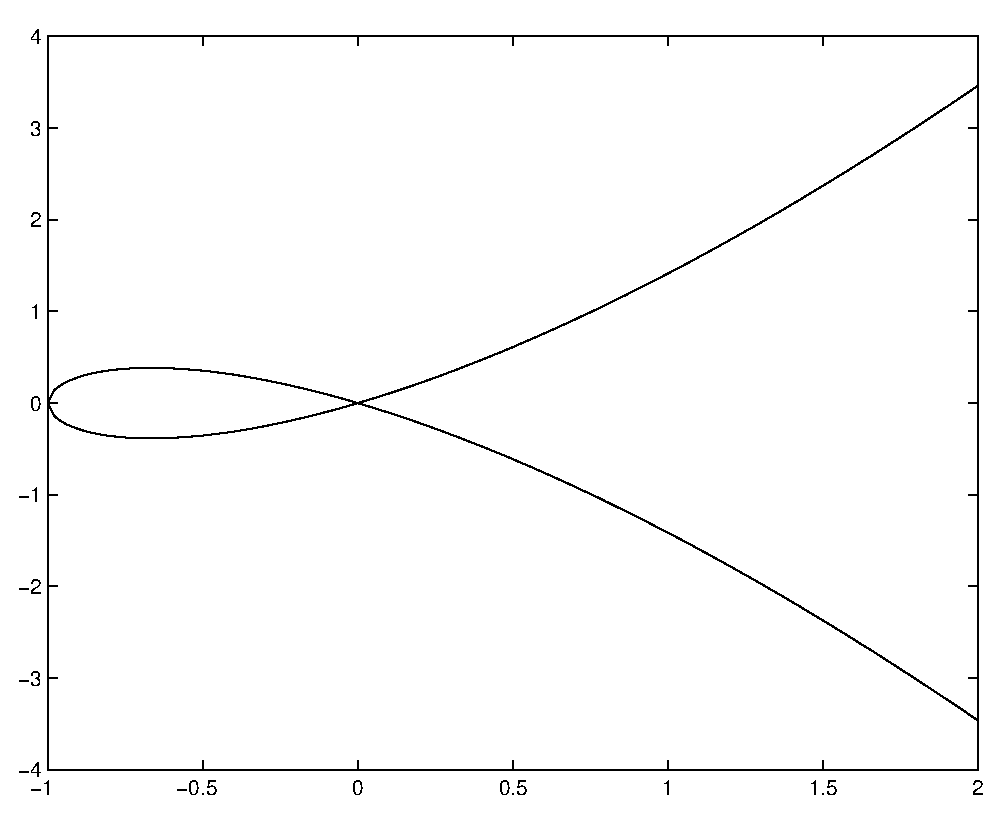
\psfig{file=exfigure/fig14-7-10.eps,width=3.0in}}
        \exercap{c14.7.10}
\end{figure} 

 